\DiaryEntry{Relations between Random Variables}{2016-01-03}{Stochastic}

\subsection{RVs with different Distribution}

Consider two RVs \(X_1, X_2\) which are independently distributed with
pdfs \(f_1(u)\), \(f_2(u)\) and cdfs
\(F_1(u) = \int_{-\infty}^u f_1(v)dv\) and
\(F_2(u) = \int_{-\infty}^u f_2(v)dv\).

We want to calculate the probability that \(X_1 < X_2\):

\[
P(X_1 < X_2) = \int_\alpha P(X_1<\alpha, X_2=\alpha) d\alpha = \int_\alpha F_1(\alpha) f_2(\alpha) d\alpha
\]

\subsubsection{Example: Two Uniform Distributions}

Consider \(X_1\) distributed uniformly on \([0,2]\) and \(X_2\)
distributed uniformly on \([1,3]\). The Figure below shows the cdf
\(F_1(u)\) in red and the pdf \(f_2(u)\) in green:

\begin{figure}[H]
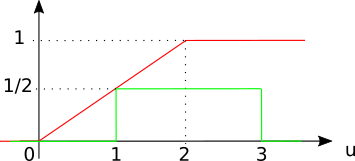
\includegraphics{images/rv_relation_1.png}
\end{figure}

The desired probability then becomes

\[
P(X_1 < X_2) = \int_\alpha F_1(\alpha) f_2(\alpha) d\alpha = \int_{\alpha=1}^{2} \frac{\alpha}{2} \frac{1}{2} d\alpha + \int_{\alpha=2}^{3} 1 \frac{1}{2} d\alpha = \frac{7}{8}
\]

\subsection{RVs with same Distribution}

In the special case that both RVs are distributed the same; i.e.~with
pdf \(f_x(u)\) and cdf \(F_x(u) = \int_{-\infty}^u f_x(v)dv\), the
probability that \(X_1 < X_2\) becomes:

\[
P(X_1 < X_2) = \int_\alpha P(X_1<\alpha, X_2=\alpha) d\alpha = \int_\alpha P(X_1<\alpha) P(X_2=\alpha) d\alpha = \int_\alpha F_X(\alpha) f_x(\alpha) d\alpha
\]

\subsubsection{Example: Uniform Distribution}

If \(X_1, X_2\) are distributed uniformly between 0 and 1, the cdf in
the interval \([0,1]\) becomes \(F_x(u) = u\) and we have

\[
P(X_1 < X_2) = \int_{\alpha=0}^1 \alpha 1 d\alpha = \frac{1}{2}
\]

\subsection{General Result}

This result holds in general; i.e.~for two RVs distributed with the same
pdf, we have \(P(X_1 < X_2) = 1/2\). This can be shown as follows:

\[
P(X_1 < X_2) = \int_{\alpha=-\infty}^\infty F(\alpha) f(\alpha) d\alpha = \int_{\alpha=-\infty}^\infty \int_{u=-\infty}^\alpha f(u) du f(\alpha) d\alpha
\]

Reordering the integrals, we obtain

\[
P(X_1 < X_2) = \int_{\alpha=-\infty}^\infty \int_{u=-\infty}^\alpha f(u) f(\alpha) du d\alpha
\]

Note that the integral over the complete \(\alpha - u\) area yields
\(1\) because we integrate over a (joint) probability function. The
integration region in the double integral above is half the area (see
Figure below), the integrand is rotational symmetric and therefore the
integral yields a value of 1/2.

\begin{figure}[H]

\includegraphics{images/rv_relation_2.png}
\end{figure}

\subsubsection{Conjecture}

$P(X_1 <  X_2) = 1/2$ holds for any two RVs with zero mean and symmetry around the origin.


%%% Local Variables:
%%% mode: latex
%%% TeX-master: "journal"
%%% End:
